\documentclass{beamer}\usepackage{graphicx, color}
%% maxwidth is the original width if it is less than linewidth
%% otherwise use linewidth (to make sure the graphics do not exceed the margin)
\makeatletter
\def\maxwidth{ %
  \ifdim\Gin@nat@width>\linewidth
    \linewidth
  \else
    \Gin@nat@width
  \fi
}
\makeatother

\IfFileExists{upquote.sty}{\usepackage{upquote}}{}
\definecolor{fgcolor}{rgb}{0.2, 0.2, 0.2}
\newcommand{\hlnumber}[1]{\textcolor[rgb]{0,0,0}{#1}}%
\newcommand{\hlfunctioncall}[1]{\textcolor[rgb]{0.501960784313725,0,0.329411764705882}{\textbf{#1}}}%
\newcommand{\hlstring}[1]{\textcolor[rgb]{0.6,0.6,1}{#1}}%
\newcommand{\hlkeyword}[1]{\textcolor[rgb]{0,0,0}{\textbf{#1}}}%
\newcommand{\hlargument}[1]{\textcolor[rgb]{0.690196078431373,0.250980392156863,0.0196078431372549}{#1}}%
\newcommand{\hlcomment}[1]{\textcolor[rgb]{0.180392156862745,0.6,0.341176470588235}{#1}}%
\newcommand{\hlroxygencomment}[1]{\textcolor[rgb]{0.43921568627451,0.47843137254902,0.701960784313725}{#1}}%
\newcommand{\hlformalargs}[1]{\textcolor[rgb]{0.690196078431373,0.250980392156863,0.0196078431372549}{#1}}%
\newcommand{\hleqformalargs}[1]{\textcolor[rgb]{0.690196078431373,0.250980392156863,0.0196078431372549}{#1}}%
\newcommand{\hlassignement}[1]{\textcolor[rgb]{0,0,0}{\textbf{#1}}}%
\newcommand{\hlpackage}[1]{\textcolor[rgb]{0.588235294117647,0.709803921568627,0.145098039215686}{#1}}%
\newcommand{\hlslot}[1]{\textit{#1}}%
\newcommand{\hlsymbol}[1]{\textcolor[rgb]{0,0,0}{#1}}%
\newcommand{\hlprompt}[1]{\textcolor[rgb]{0.2,0.2,0.2}{#1}}%

\usepackage{framed}
\makeatletter
\newenvironment{kframe}{%
 \def\at@end@of@kframe{}%
 \ifinner\ifhmode%
  \def\at@end@of@kframe{\end{minipage}}%
  \begin{minipage}{\columnwidth}%
 \fi\fi%
 \def\FrameCommand##1{\hskip\@totalleftmargin \hskip-\fboxsep
 \colorbox{shadecolor}{##1}\hskip-\fboxsep
     % There is no \\@totalrightmargin, so:
     \hskip-\linewidth \hskip-\@totalleftmargin \hskip\columnwidth}%
 \MakeFramed {\advance\hsize-\width
   \@totalleftmargin\z@ \linewidth\hsize
   \@setminipage}}%
 {\par\unskip\endMakeFramed%
 \at@end@of@kframe}
\makeatother

\definecolor{shadecolor}{rgb}{.97, .97, .97}
\definecolor{messagecolor}{rgb}{0, 0, 0}
\definecolor{warningcolor}{rgb}{1, 0, 1}
\definecolor{errorcolor}{rgb}{1, 0, 0}
\newenvironment{knitrout}{}{} % an empty environment to be redefined in TeX

\usepackage{alltt}
\usepackage[]{graphicx, parskip, microtype, hyperref}

\frenchspacing

\usetheme{default}
\usecolortheme{orchid}




\title{ggplot2: a philosophy and a package}
\author{Peter D Smits}
\institute{Committee on Evolutionary Biology \\
University of Chicago}
\date{\today}

\begin{document}

\begin{frame}
  \maketitle
\end{frame}

\begin{frame}
  \frametitle{Introduction}

  there are three main ways of making graphics in R:\\
  base graphics, lattice, grid, ggplot2.

  ggplot2 is an R package written (primarily) by Hadley Wickham.

  implementation of the Grammar of Graphics (by Leland Wilkinson).

  extremely popular, huge community, extremely powerful.

\end{frame}

\begin{frame}
  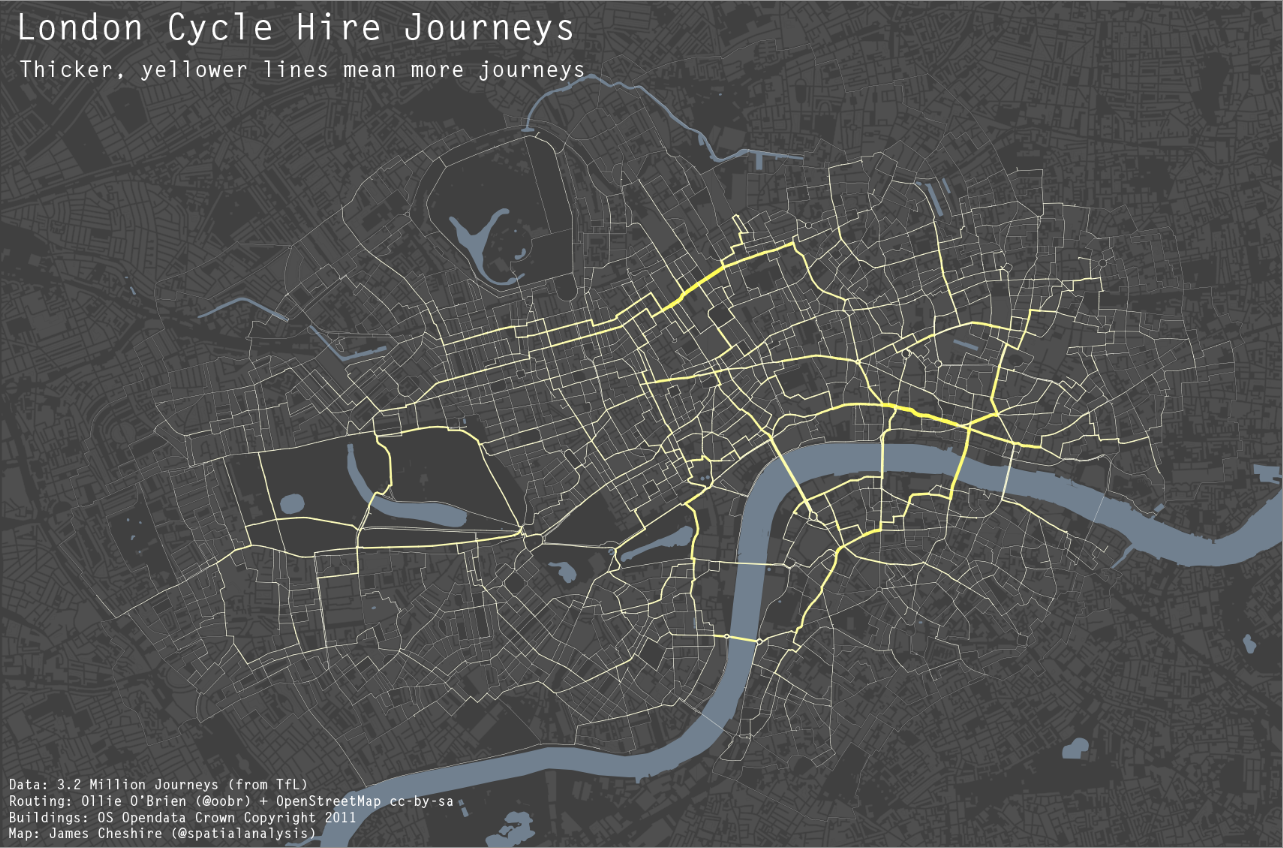
\includegraphics[width = \textwidth, keepaspectratio = true]{figure/bike_ggplot}

\end{frame}

\begin{frame}
  \frametitle{Hadley Wickham}

  \begin{columns}
    \begin{column}{0.5\textwidth}
      \begin{itemize}
        \item professor of statistics at Rice University
        \item from New Zealand (oddly common in statistics)
        \item author of many R packages (ggplot2, reshape2, plyr, devtools, and more)
        \item ggplot and reshape made up most of his PhD thesis
      \end{itemize}
    \end{column}
    \begin{column}{0.5\textwidth}
      
\includegraphics[width = \textwidth, keepaspectratio = true]{figure/hw}
    \end{column}
  \end{columns}

\end{frame}

\begin{frame}
  \frametitle{Grammar of Graphics}
  \begin{columns}
    \begin{column}{0.5\textwidth}
      most texts on graphics were written a while ago (Tukey '77, Tufte '83, Chambers et al. '83, Cleveland '85). GoG newer and more ``modern''.
      \\~\\
      few basic ideas
      \begin{itemize}
        \item variables
        \item aesthetics
        \item geometry
        \item statistics
        \item facets
        \item scales, etc.
      \end{itemize}
    \end{column}
    \begin{column}{0.5\textwidth}
      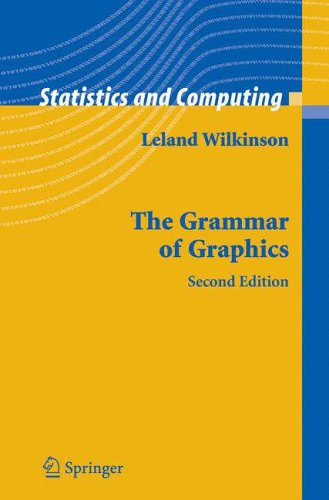
\includegraphics[width = \textwidth, keepaspectratio = true]{figure/grammar}
    \end{column}
  \end{columns}

\end{frame}

\begin{frame}
  \frametitle{Basic implementation}
  \begin{itemize}
    \item object (ggplot)
    \item aesthetics (aes)
      \begin{itemize}
        \item x, y position
        \item size, shape
        \item group, colour
      \end{itemize}
    \item geometrics (geom) and statistics (stat)
      \begin{itemize}
        \item points, lines, line segments
        \item bars, histograms, boxes
        \item maps (!!)
        \item and more
      \end{itemize}
    \item themes
  \end{itemize}

\end{frame}

\begin{frame}
  \frametitle{Today's first data}

  The muscle car data set!

  mtcars (part of base R install, along with a lot of other datasets)

  11 cars for 32 variables. Below is tiny subset.

\begin{kframe}


{\ttfamily\noindent\itshape\textcolor{messagecolor}{\#\# Loading required package: xtable}}\end{kframe}% latex table generated in R 2.15.2 by xtable 1.7-0 package
% Sun Jan  6 00:09:10 2013
\begin{table}[ht]
\begin{center}
\begin{tabular}{rrrrrrr}
  \hline
 & mpg & cyl & disp & hp & drat & wt \\ 
  \hline
Mazda RX4 & 21.00 & 6.00 & 160.00 & 110.00 & 3.90 & 2.62 \\ 
  Mazda RX4 Wag & 21.00 & 6.00 & 160.00 & 110.00 & 3.90 & 2.88 \\ 
  Datsun 710 & 22.80 & 4.00 & 108.00 & 93.00 & 3.85 & 2.32 \\ 
  Hornet 4 Drive & 21.40 & 6.00 & 258.00 & 110.00 & 3.08 & 3.21 \\ 
  Hornet Sportabout & 18.70 & 8.00 & 360.00 & 175.00 & 3.15 & 3.44 \\ 
  Valiant & 18.10 & 6.00 & 225.00 & 105.00 & 2.76 & 3.46 \\ 
   \hline
\end{tabular}
\end{center}
\end{table}



\end{frame}

\begin{frame}[fragile]
  \frametitle{Our first graph}
\begin{knitrout}
\definecolor{shadecolor}{rgb}{0.969, 0.969, 0.969}\color{fgcolor}\begin{kframe}
\begin{alltt}
\hlfunctioncall{library}(ggplot2)
g1 <- \hlfunctioncall{ggplot}(mtcars, \hlfunctioncall{aes}(wt, mpg)) + \hlfunctioncall{geom_point}()
g1
\end{alltt}
\end{kframe}
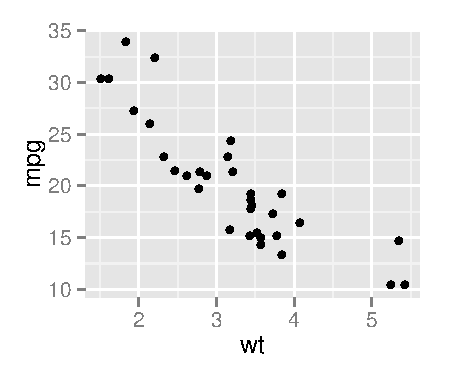
\includegraphics[width=\maxwidth]{figure/first} 

\end{knitrout}


\end{frame}

\begin{frame}[fragile]
  \frametitle{Adding a stat and modifying our first graph}
\begin{knitrout}
\definecolor{shadecolor}{rgb}{0.969, 0.969, 0.969}\color{fgcolor}\begin{kframe}
\begin{alltt}
g1 <- g1 + \hlfunctioncall{stat_smooth}(method = \hlstring{"lm"})
g1 <- g1 + \hlfunctioncall{geom_point}(\hlfunctioncall{aes}(colour = \hlfunctioncall{factor}(cyl)))
g1
\end{alltt}
\end{kframe}
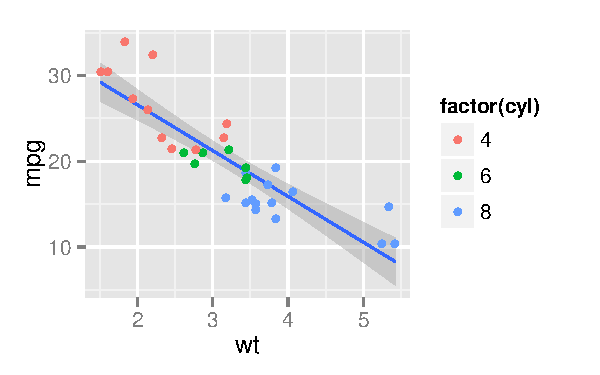
\includegraphics[width=\maxwidth]{figure/first-modify} 

\end{knitrout}


\end{frame}

\begin{frame}[fragile]
  \frametitle{Try and make it look prettier}
\begin{knitrout}\scriptsize
\definecolor{shadecolor}{rgb}{0.969, 0.969, 0.969}\color{fgcolor}\begin{kframe}
\begin{alltt}
g1 <- g1 + \hlfunctioncall{theme}(legend.position = \hlstring{'none'},
                 axis.line = \hlfunctioncall{element_line}(colour = \hlstring{'black'}),
                 panel.background = \hlfunctioncall{element_blank}())
g1
\end{alltt}
\end{kframe}
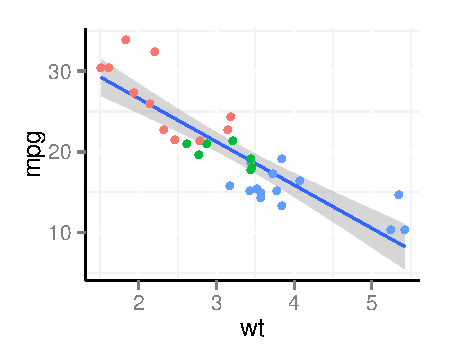
\includegraphics[width=\maxwidth]{figure/first-line} 

\end{knitrout}

\end{frame}

\begin{frame}[fragile]
  \frametitle{Our second graph}
\begin{knitrout}
\definecolor{shadecolor}{rgb}{0.969, 0.969, 0.969}\color{fgcolor}\begin{kframe}
\begin{alltt}
g2 <- \hlfunctioncall{ggplot}(mtcars, 
             \hlfunctioncall{aes}(x = \hlfunctioncall{factor}(cyl), 
                 y = mpg, 
                 fill = \hlfunctioncall{factor}(cyl)))
g2 <- g2 + \hlfunctioncall{geom_boxplot}()
g2 <- g2 + \hlfunctioncall{theme}(legend.position = \hlstring{'none'},
                 panel.background = \hlfunctioncall{element_blank}(),
                 panel.grid = \hlfunctioncall{element_blank}())
g2 <- g2 + \hlfunctioncall{labs}(x = \hlstring{'cylinders'}, 
                y = \hlstring{'miles per gallon'},
                title = \hlstring{'example box plot'})
\end{alltt}
\end{kframe}
\end{knitrout}


\end{frame}

\begin{frame}[fragile]
  \frametitle{Our second graph}
\begin{knitrout}
\definecolor{shadecolor}{rgb}{0.969, 0.969, 0.969}\color{fgcolor}
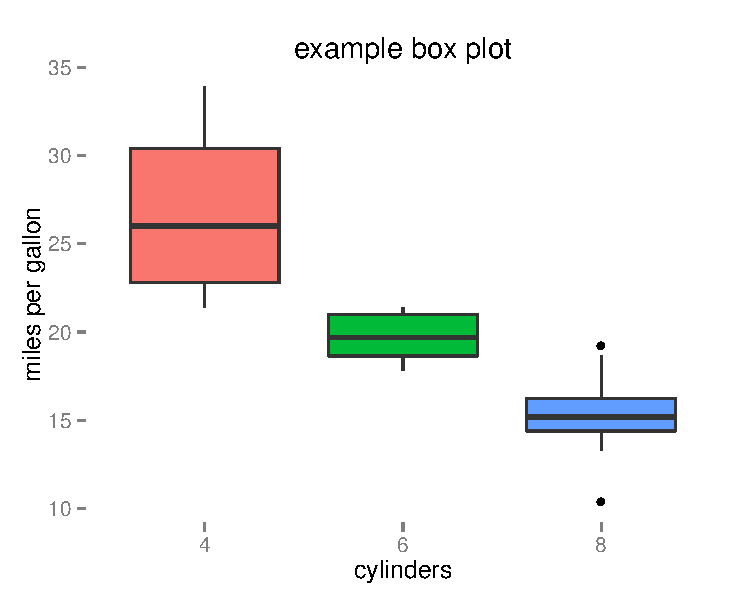
\includegraphics[width=\maxwidth]{figure/second-plot} 

\end{knitrout}


\end{frame}

\begin{frame}
  \frametitle{Today's second dataset}

  diamonds!

  53940 samples for 10 variables.

  Here is a tiny part of that dataset.

% latex table generated in R 2.15.2 by xtable 1.7-0 package
% Sun Jan  6 00:09:12 2013
\begin{table}[ht]
\begin{center}
\begin{tabular}{rrlllrrr}
  \hline
 & carat & cut & color & clarity & depth & table & price \\ 
  \hline
1 & 0.23 & Ideal & E & SI2 & 61.50 & 55.00 & 326 \\ 
  2 & 0.21 & Premium & E & SI1 & 59.80 & 61.00 & 326 \\ 
  3 & 0.23 & Good & E & VS1 & 56.90 & 65.00 & 327 \\ 
  4 & 0.29 & Premium & I & VS2 & 62.40 & 58.00 & 334 \\ 
  5 & 0.31 & Good & J & SI2 & 63.30 & 58.00 & 335 \\ 
  6 & 0.24 & Very Good & J & VVS2 & 62.80 & 57.00 & 336 \\ 
   \hline
\end{tabular}
\end{center}
\end{table}



\end{frame}

\begin{frame}[fragile]
  \frametitle{Looking at diamonds}
\begin{knitrout}
\definecolor{shadecolor}{rgb}{0.969, 0.969, 0.969}\color{fgcolor}\begin{kframe}
\begin{alltt}
d <- \hlfunctioncall{ggplot}(diamonds, 
            \hlfunctioncall{aes}(x = carat, y = price, 
                colour = clarity))
d <- d + \hlfunctioncall{geom_point}()
d
\end{alltt}
\end{kframe}
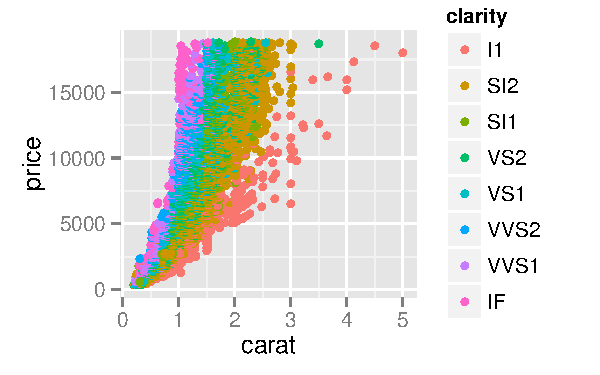
\includegraphics[width=\maxwidth]{figure/dia} 

\end{knitrout}


\end{frame}

\begin{frame}[fragile]
  \frametitle{Make that look better}
\begin{knitrout}
\definecolor{shadecolor}{rgb}{0.969, 0.969, 0.969}\color{fgcolor}\begin{kframe}
\begin{alltt}
d <- d + \hlfunctioncall{geom_point}(alpha = 0.1)
d <- d + \hlfunctioncall{facet_wrap}(~ color)
\end{alltt}
\end{kframe}
\end{knitrout}


\end{frame}

\begin{frame}
\begin{knitrout}
\definecolor{shadecolor}{rgb}{0.969, 0.969, 0.969}\color{fgcolor}
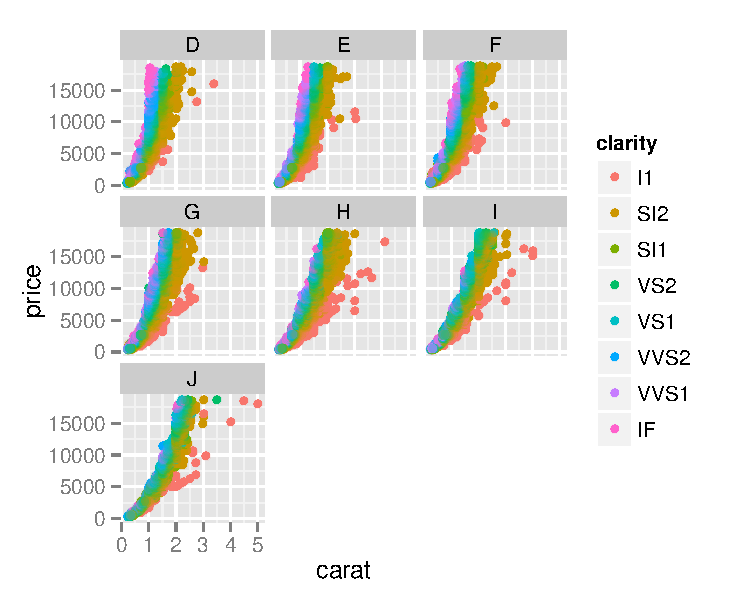
\includegraphics[width=\maxwidth]{figure/dia2-plot} 

\end{knitrout}

\end{frame}<++>


\begin{frame}
  \frametitle{Other useful packages}

  GGally: matrix plots

  ggthemes: various canned themes to make your plots prettier (or hilariously ugly)

\end{frame}

\begin{frame}
  \frametitle{Useful websites}

  \url{http://docs.ggplot2.org/current/} : current ggplot documentation (very good)

  \url{http://groups.google.com/group/ggplot2} : ggplot2 mailing list

  \url{http://wiki.stdout.org/rcookbook/Graphs} : various tips and tricks to get over problems

  \url{http://stackoverflow.com/} : coding question/answer site

  \url{http://stats.stackexchange.com/} : statistics question/answer site

  \url{http://www.r-bloggers.com/} : R blog aggregator

\end{frame}


\end{document}
